
\section{Processes and Threads}
\label{sec:orgheadline7}
ref : \href{https://developer.android.com/guide/components/processes-and-threads.html}{link: dev > API Guides > App Components > Processes and Threads}

By default, all components of the same application run in the same process and
thread (called the "main" thread). However, you can arrange for different
components in your application to run in separate processes, and you can
create additional threads for any process.

\subsection{Processes}
\label{sec:orgheadline1}
In manifest file, each type of component element (e.g. \texttt{<activity>}) and
\texttt{<application>} supports an \texttt{android:process} attribute that can specify a
process in which that component should run.

\subsection{Threads}
\label{sec:orgheadline4}
A main thread is created when an application is launched. THsi thread is in
charge of dispatching events to UI widgets and interactions with UI
components from the Android UI toolkit. As such, the main thread is also
called the UI thread.

There are two rules to Android's single thread model:
\begin{enumerate}
\item Do not block the UI thread. no events can be dispathed (including drawing)
when blocked. blocking 5 seconds causes "application not responding",
\item Do not access the Android UI toolkit from outside the UI thread. they are
not thread-safe.
\end{enumerate}

\subsubsection{Worker threads}
\label{sec:orgheadline2}
Do blocking task in a new \texttt{Thread} and post UI update operations by methods
such as \texttt{Activity.runOnUiThread(Runnable)} , \texttt{View.post(Runnable)},
\texttt{View.postDelayed(Runnable, long)}. Or use \texttt{AsyncTask} to make this process
esaier.

\subsubsection{{\bfseries\sffamily TODO} Thread-safe methods}
\label{sec:orgheadline3}

\subsection{{\bfseries\sffamily TODO} Interproceess Communication}
\label{sec:orgheadline5}
Android offers a mechanism for interprocess communication (IPC) using remote
procedure calls (RPCs), in which a method is called by an activity or other
application component, but executed remotely (in another process), with any
result returned back to the caller. Data must be understood by the operating
system to be moved from the address space of one process to another.


\subsection{Other Event based libaraies}
\label{sec:orgheadline6}
ref : \href{http://wale.oyediran.me/2015/07/16/event-driven-android/}{blog: Event Driven Android}

\begin{itemize}
\item \href{http://greenrobot.github.io/EventBus/}{github: EventBus} Android optimized event bus that simplifies communication
between Activities, Fragments, Threads, Services, etc.
\item \href{http://square.github.io/otto/}{github: Otto} An enhanced event bus with emphasis on Android support
\end{itemize}


\section{Lifecycle of components}
\label{sec:orgheadline9}

ref : \href{https://developer.android.com/guide/topics/processes/process-lifecycle.html}{link: dev > API Guides > Process-lifecycle}

"It is important that application developers understand how different
application components (in particular Activity, Service, and
BroadcastReceiver) impact the lifetime of the application's process. Not using
these components correctly can result in the system killing the application's
process while it is doing important work."

\textbf{lifecycle bugs}



\subsection{Activity}

ref : \href{https://developer.android.com/guide/components/activities/activity-lifecycle.html}{link: dev > API Guides > App Components > Activities}

\begin{wrapfigure}[20]{r}{0.5\textwidth}
  % \centering
  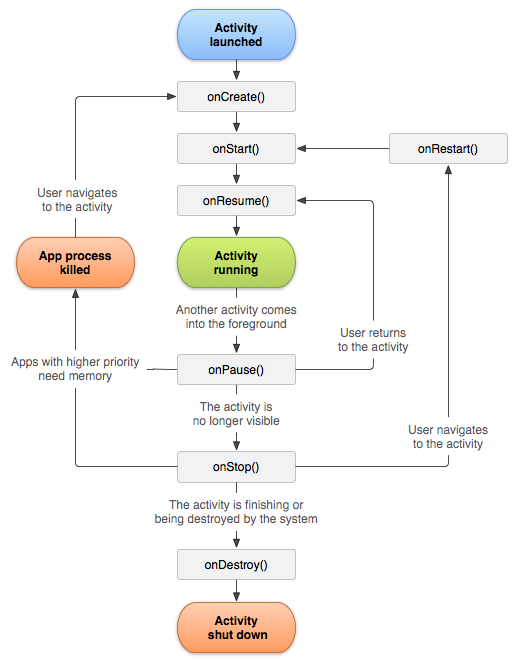
\includegraphics[width=.5\textwidth]{img/activity_lifecycle}
  \caption{The Lifecycle of Activity}
\end{wrapfigure}

For example, good implementation of the lifecycle callbacks can help ensure
that your app avoids:
\begin{itemize}
\item Crashing if the user receives a phone call or switches to another app
  while using your app.
\item Consuming valuable system resources when the user is not actively using
  it.
\item Losing the user's progress if they leave your app and return to it at a
  later time.
\item Crashing or losing the user's progress when the screen rotates between
  landscape and portrait orientation.
\end{itemize}


The \emph{entire lifetime} is between \texttt{onCreate()} and
\texttt{onDestroy()}. The \emph{visible lifetime} is between
\texttt{onStart()} and \texttt{onStop()}. The \emph{foreground lifetime} is
between \texttt{onResume()} and \texttt{onPause()}

Activity is a class. User extends this class will implement \texttt{onCreate()}
to do their initial setup. You should always call up to your superclass when
implementing these methods.

\subsubsection{Starting Activities and Getting Results}

\begin{itemize}
\item \texttt{startActvity(Intent)} : start an activity on the top of the
  activity stack, \texttt{Intent} describes the activity to be executed.
\item \texttt{startActvitiyForResult(Intent, int)} : start an activity with a
  second integer parameter identifying the call.
\item \texttt{onActivityResult(int, int, Intent)} : callback where you get the
  result.
\item \texttt{setResult(int)} : use this to return data
\end{itemize}

\subsubsection{Process Lifecycle Based on Activity Lifecycle}
\begin{enumerate}
\item \textbf{Foreground activity} : visible, interactive
\item \textbf{Visible activity} : visible, not interactive, such as one sitting
  behind a foreground dialog.
\item \textbf{Backfround activity} : invisible, so the system may safely kill
  its process to reclaim memory.
\item \textbf{Empty process} : a process hosting no activites or other
  application components.
\end{enumerate} 


\subsection{Service}

% ref : \href{https://developer.android.com/reference/android/app/Service.html}
% {link: dev > API Guides > App Components > Activities}

Service is not a separate process, neither a thread. It is running in the
application's main process unless otherwise specified. Service is a facility for
the application to tell the system about something it wants to be doing in the
background to expose some of its functionality to other apps.



\subsection{Content Providers}








  




